\clearpage
\setcounter{page}{1}

% Uncomment this if you want to follow the CVPR template
% \maketitlesupplementary
% Use this for arxiv
\appendix

\twocolumn[{%
\centering
\setlength{\tabcolsep}{6pt}
\renewcommand{\arraystretch}{1.3}
\begin{tabular}{lccccc}
    \toprule
    Video len. & Ctx. len & Trainable parameters & Learning rate & Schedule & Steps \\
    \midrule
    3 sec & 18048 & TTT / Pre-trained Params & $1 \times 10^{-4}$ / $1\times 10^{-5}$ & Cosine / Constant & 5000 \\
    9 sec & 51456 & TTT + Local Attn (QKVO) & $1 \times 10^{-5}$ & Constant & 5000 \\
    18 sec & 99894 & TTT + Local Attn (QKVO) & $1 \times 10^{-5}$ & Constant & 1000 \\
    30 sec & 168320 & TTT + Local Attn (QKVO) & $1 \times 10^{-5}$ & Constant & 500 \\
    63 sec & 341550 & TTT + Local Attn (QKVO) & $1 \times 10^{-5}$ & Constant & 250 \\
    \bottomrule
\end{tabular}
\captionof{table}{Hyper-parameters for multi-stage fine-tuning. First, the entire pre-trained model is fine-tuned on 3-second segments of \textit{Tom and Jerry}, with higher learning rates assigned to the newly introduced TTT layers and gates. Then, only TTT layers, gates, and self-attention parameters are fine-tuned at reduced learning rates.}
\label{tab:appendix:hparams}
\vspace{1em}

\begin{tabular}{lcccc|c}
    \toprule
     & Text following & Motion naturalness & Aesthetics & Temporal consistency & Average \\
    \midrule
    {Local Attention} & 965 & 972 & 969 & 944 & 962 \\
    {TTT-Linear} & 1003 & 995 & 1007 & 1001 & 1001 \\
    {Mamba 2} & \textbf{1023} & 987 & 1008 & 1004 & 1005 \\
    {Gated DeltaNet} & 1020 & \textbf{1039} & \textbf{1044} & {1026} & \textbf{1032} \\
    {SWA} & 995 & 1004 & 993 & 980 & 993 \\
    {TTT-MLP} & 994 & 1002 & 1002 & 1019 & 1004 \\
    \bottomrule
\end{tabular}
\captionof{table}{Human evaluation results for 18-second videos, discussed in Subsection~\ref{subsec:results} and \ref{subsec:limitations}.}
\label{tab:appendix:multiaxis_evaluation}
\vspace{1em}
}]

% \twocolumn[{
% \centering
% \setlength{\tabcolsep}{6pt}
% \renewcommand{\arraystretch}{1.3}
% \begin{tabular}{cccccc}
%     \toprule
%     \textbf{Video Len.} & \textbf{Ctx. Len.} & \textbf{Trainable Parameters} & \textbf{LR} & \textbf{Schedule} & \textbf{Steps} \\
%     \midrule
%     3 sec & 18048 & TTT / Pre-trained Params & $1 \times 10^{-4}$ / $1\times 10^{-5}$ & Cosine / Constant & 5000 \\
%     9 sec & 51456 & TTT + Local Attn (QKVO) & $1 \times 10^{-5}$ & Constant & 5000 \\
%     18 sec & 99894 & TTT + Local Attn (QKVO) & $1 \times 10^{-5}$ & Constant & 1000 \\
%     30 sec & 168320 & TTT + Local Attn (QKVO) & $1 \times 10^{-5}$ & Constant & 500 \\
%     63 sec & 341550 & TTT + Local Attn (QKVO) & $1 \times 10^{-5}$ & Constant & 250 \\
%     \bottomrule
% \end{tabular}
% \captionof{table}{Model configurations for multi-stage fine-tuning. First, the entire pre-trained model is fine-tuned on 3-second segments of \textit{Tom and Jerry}, with higher learning rates assigned to the newly introduced TTT layers and gates. Then, only TTT layers, gates, and self-attention parameters are fine-tuned at reduced learning rates.}
% \label{tab:appendix:hparams}
% \vspace{1em}
% }]

% \begin{figure*}[h]
%     \centering
%     \begin{minipage}{\textwidth}
%       \centering
%       % \renewcommand{\arraystretch}{1.2}
%       \begin{tabular}{lcccc|c}
%         \toprule
%          & Text following & Motion naturalness & Aesthetics & Temporal consistency & Average \\
%         \midrule
%         {Local Attention} & 965 & 972 & 969 & 944 & 962 \\
%         {TTT-Linear} & 1003 & 995 & 1007 & 1001 & 1001 \\
%         {Mamba 2} & \textbf{1023} & 987 & 1008 & 1004 & 1005 \\
%         {Gated DeltaNet} & 1020 & \textbf{1039} & \textbf{1044} & {1026} & \textbf{1032} \\
%         {SWA} & 995 & 1004 & 993 & 980 & 993 \\
%         {TTT-MLP} & 994 & 1002 & 1002 & 1019 & 1004 \\
%         \bottomrule
%       \end{tabular}
%       \captionof{table}{Human evaluation results for 18-second videos.}
%       \label{tab:appendix:multiaxis_evaluation}
%       \vspace{1em}
%     \end{minipage}
% \end{figure*}

\section{Experiment Details}
\label{sec:appendix:implementation}

\myparagraph{Diffusion schedule.} 
Following CogVideoX~\cite{yang2024cogvideox}, we fine-tune our model using v-prediction~\cite{salimans2022progressive}, which includes a diffusion noise schedule with 1000 steps and Zero-SNR~\cite{lin2024zerosnr} enforced at the final step.

\myparagraph{Training configurations.} We use the following hyper-parameters for all stages of training:

\vspace{0.2em}
\begin{itemize}[itemsep=0.2em]
    \item \textbf{Optimizer:} AdamW with $(\beta_1, \beta_2) = (0.9, 0.95)$
    \item \textbf{Learning Rate:} Linear warmup over 2\% of training steps
    \item \textbf{Batch Size:} 64
    \item \textbf{Gradient Clipping:} 0.1
    \item \textbf{Weight Decay:} $10^{-4}$ applied to all params except biases and normalization layers
    \item \textbf{VAE Scale Factor}: 1.0
    \item \textbf{Dropout:} Zero-out text prompt with probability 0.1
    \item \textbf{Precision:} Mixed Precision with PyTorch FSDP2
\end{itemize}

\myparagraph{TTT configurations.} A key hyperparameter for TTT layers is the inner-loop learning rate $\eta$, which we set $\eta = 1.0$ for TTT-Linear and $\eta = 0.1$ for TTT-MLP.

\myparagraph{Sampling schedule.} We follow the DDIM sampler~\cite{song2021ddim} with 50 steps, applying dynamic classifier-free guidance (CFG)~\cite{ho2022cfg} that increases CFG magnitude from 1 to 4 and utilizing negative prompts to further enhance video quality.

\section{On-Chip Tensor Parallel Details}
\label{sec:appendix:systems}

We use ThunderKittens~\cite{spector2025thunderkittens} to implement the TTT-MLP kernel, described in Subsection \ref{subsec:gpu}.

\vspace{0.75em} \myparagraph{Hidden state sharding.} We follow the standard strategy for Tensor Parallel, sharding the first layer column-wise and the second layer row-wise. As the GeLU non-linearity is elementwise, the forward pass of the TTT-layer requires a single reduction for computing the inner loss used to update the hidden state.

\myparagraph{Further latency optimizations.} We incorporate several techniques from FlashAttention-3 \cite{shah2024flashattention3fastaccurateattention} to further reduce I/O latency on NVIDIA Hopper GPUs. In particular, we implement a multi-stage pipelining scheme that asynchronously prefetches future mini-batches from HBM, overlapping data transfers with computation on the current mini-batch. This approach, known as \textit{producer-consumer asynchrony}, involves dedicating specialized warpgroups to either data loading (producer) or computation (consumer).

\myparagraph{Gradient checkpointing.}
We integrate gradient checkpointing along the sequence dimension~\cite{sun2024ttt} directly into our fused kernel. To reduce I/O-induced stalls and CUDA thread workloads, we use the Tensor Memory Accelerator (TMA) to perform asynchronous memory stores.

\begin{figure*}[!t]
    \centering
    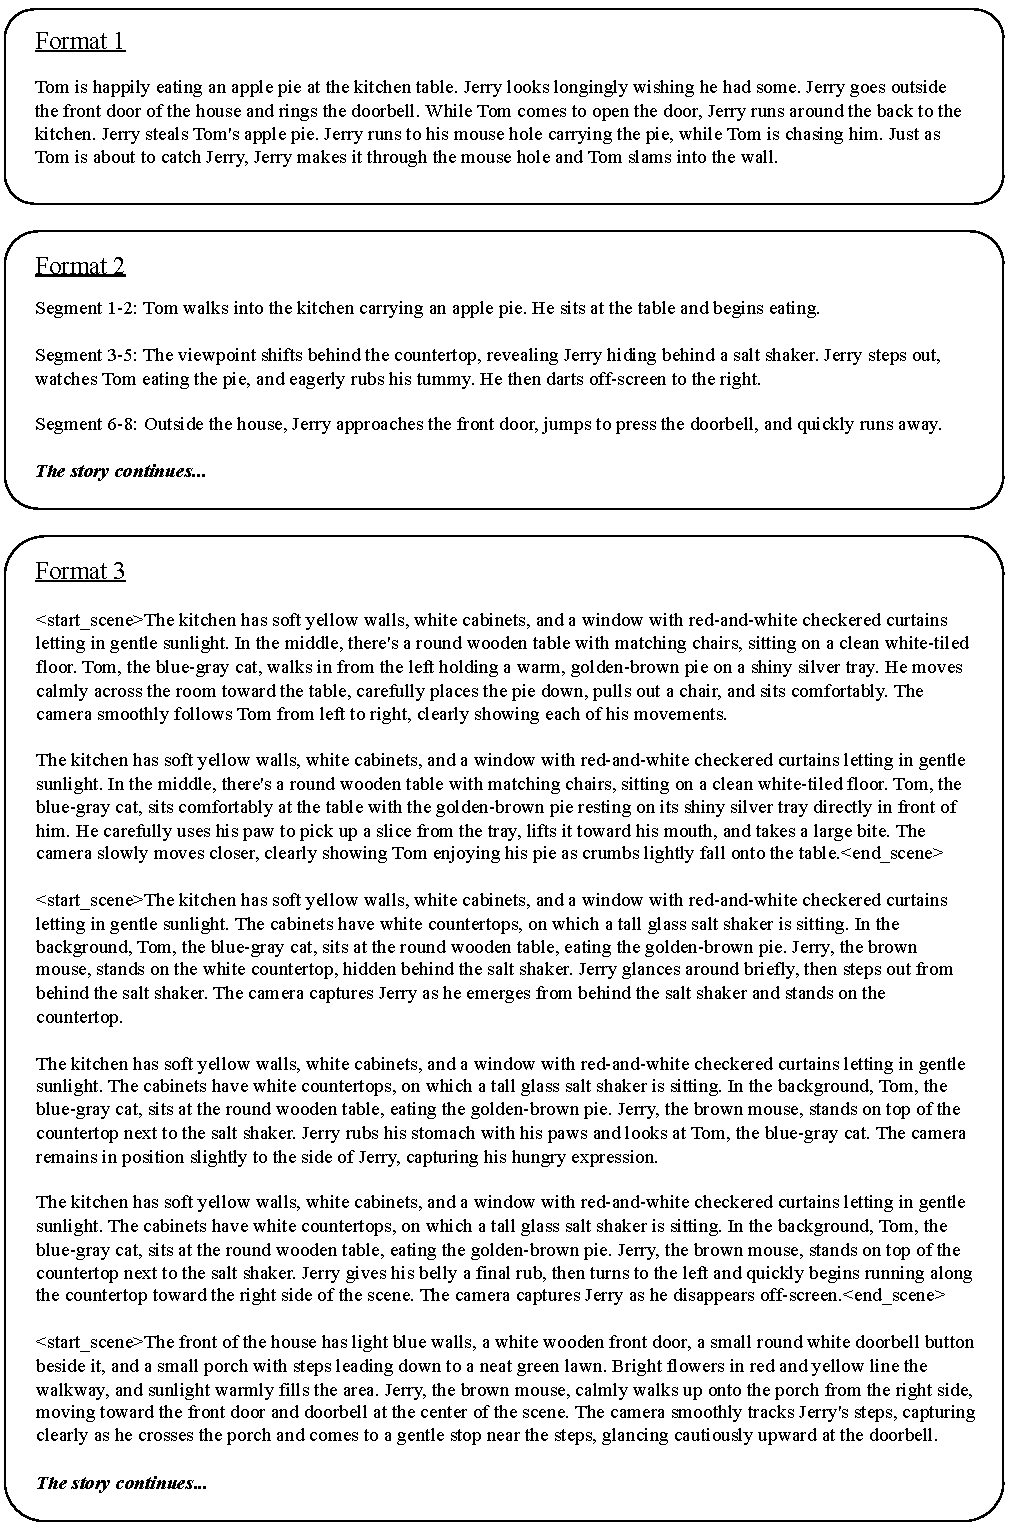
\includegraphics[width=0.82\textwidth]{figs/prompt.pdf}
    \caption{Illustration of the three prompt formats discussed in Subsection~\ref{subsec:pipeline}: (1) a short summary of the plot, (2) sentence-level descriptions of the segments, and (3) a detailed storyboard.}
    \label{fig:prompts}
\end{figure*}